
%%%%%%%%%%%%%%%%%%%%%%%%%%%%%%%%%%%%%%%%%
% Jacobs Landscape Poster
% LaTeX Template
% Version 1.0 (29/03/13)
%
% Created by:
% Computational Physics and Biophysics Group, Jacobs University
% https://teamwork.jacobs-university.de:8443/confluence/display/CoPandBiG/LaTeX+Poster
% 
% Further modified by:
% Nathaniel Johnston (nathaniel@njohnston.ca)
%
% This template has been downloaded from:
% http://www.LaTeXTemplates.com
%
% License:
% CC BY-NC-SA 3.0 (http://creativecommons.org/licenses/by-nc-sa/3.0/)
%
%%%%%%%%%%%%%%%%%%%%%%%%%%%%%%%%%%%%%%%%%

%----------------------------------------------------------------------------------------
%	PACKAGES AND OTHER DOCUMENT CONFIGURATIONS
%----------------------------------------------------------------------------------------

\documentclass[20pt]{beamer}

\usepackage{beamerposter} % Use the beamerposter package for laying out the poster

\usepackage{algorithm}
\usepackage{algpseudocode}
\usepackage{amsfonts}
\usepackage{amsmath}
\usepackage{amssymb}
\usepackage{amsthm}
\usepackage{caption}
\usepackage{comment}
\usepackage{dsfont} 
\usepackage{fancybox}
\usepackage{graphicx}
\usepackage{hyperref}

\usepackage{listings}
\usepackage{amssymb}
\usepackage{multirow}
\usepackage{ mathrsfs }
\usepackage{subcaption}
\usepackage[utf8]{inputenc}
\usepackage{url}

%tikz package 
\usepackage[graphicx]{realboxes}
\usepackage{tikz}
\usetikzlibrary{automata,positioning}
\usepackage{float}

%theme for conference poster
\usetheme{confposter} % Use the confposter theme supplied with this template

\newcommand{\ComputeNashBF}{\ensuremath{\textbf{\textsf{ComputeNash}}}}
\newcommand{\DSum}[2]{\mathsf{ut}(#1, #2)}



\usefonttheme{serif}
\usepackage[absolute,overlay]{textpos}
\definecolor{UniBlue}{RGB}{73,101,150}
\setbeamercolor{block title}{fg=blue,bg=white} % Colors of the block titles
\setbeamercolor{block body}{fg=black,bg=white} % Colors of the body of blocks
\setbeamercolor{block alerted title}{fg=white,bg=dblue!70} % Colors of the highlighted block titles
\setbeamercolor{block alerted body}{fg=black,bg=dblue!10} % Colors of the body of highlighted blocks
\setbeamertemplate{bibliography entry title}{}
\setbeamertemplate{bibliography entry location}{}
\setbeamertemplate{bibliography entry note}{}

%\setbeamerfont*{frametitle}{family=\rmfamily,series=\bfseries,size={\fontsize{32}{36}}}
%\setbeamerfont{block title}{size=\Large}
\captionsetup{justification=centering}
% Many more colors are available for use in beamerthemeconfposter.sty

%-----------------------------------------------------------
% Define the column widths and overall poster size
% To set effective sepwid, onecolwid and twocolwid values, first choose how many columns you want and how much separation you want between columns
% In tis template, the separation width chosen is 0.024 of the paper width and a 4-column layout
% onecolwid should therefore be (1-(# of columns+1)*sepwid)/# of columns e.g. (1-(4+1)*0.024)/4 = 0.22
% Set twocolwid to be (2*onecolwid)+sepwid = 0.464
% Set threecolwid to be (3*onecolwid)+2*sepwid = 0.708h
\newlength{\startsepwidth}
\newlength{\sepwid}
\newlength{\onecolwid}
\newlength{\twocolwid}
\newlength{\threecolwid}
\newlength{\middlecolwid}

%\setlength{\paperwidth}{48in} % A0 width: 46.8in
%\setlength{\paperheight}{36in} % A0 height: 33.1in
\setlength{\startsepwidth}{0.02\paperwidth} 

\setlength{\sepwid}{0.024\paperwidth} % Separation width (white space) between columns
\setlength{\onecolwid}{0.3\paperwidth} % Width of one column
\setlength{\middlecolwid}{0.3\paperwidth}
\setlength{\twocolwid}{0.618\paperwidth} % Width of two columns
\setlength{\threecolwid}{0.948\paperwidth} % Width of three columns
\setlength{\topmargin}{0in} % Reduce the top margin size
\setbeamerfont*{itemize/enumerate subbody}{parent=itemize/enumerate body}
\setbeamerfont*{itemize/enumerate subsubbody}{parent=itemize/enumerate body}
%\setbeamerfont*{block title}{size=\Huge}
%-----------------------------------------------------------

\usepackage{graphicx}  % Required for including images


\usepackage{booktabs} % Top and bottom rules for tables



\newcommand*{\CNN}{\ensuremath{\mathsf{CNN}}}
\newcommand*{\K}{\ensuremath{\mathsf{Kaught22}}}
\newcommand*{\keras}{\ensuremath{\mathsf{Keras}}}
\newcommand*{\numpy}{\ensuremath{\mathsf{NumPy}}}
\newcommand*{\scipy}{\ensuremath{\mathsf{SciPy}}}
\newcommand*{\scikit}{\ensuremath{\mathsf{sckit-learn}}}
\newcommand*{\Theano}{\ensuremath{\mathsf{Theano}}}
\newcommand*{\Model}[1]{\ensuremath{\mathsf{Model}}:#1}

%----------------------------------------------------------------------------------------
%	TITLE SECTION 
%----------------------------------------------------------------------------------------

\title{{\Huge \textsf{$\K$ for image classification}}} % Poster title

\author{{\huge \textsf{Team Katch22: Harsh Upadhyay (hu3), Suguman Bansal (sb55)}}}
\institute{{\huge \textsf{COMP540: Rice University}}}


%----------------------------------------------------------------------------------------

\begin{document}


%\begin{textblock}{3}(0.2,0.1)
%\small{
%\textcolor{blue}{
%ExCAPE Annual Meeting\\
%June 10-11, 2013}
%}
%\end{textblock}
\begin{textblock}{16}(0.2,0.5)

\includegraphics[width=12cm]{Images/Rice_logo.png}
\end{textblock}
\addtobeamertemplate{block end}{}{\vspace*{1ex}} 
% White space under blocks
\addtobeamertemplate{block alerted end}{}{\vspace*{0ex}} % White space under highlighted (alert) blocks

\setlength{\belowcaptionskip}{2ex} % White space under figures
\setlength\belowdisplayshortskip{2ex} % White space under equations


\begin{frame}[t] % The whole poster is enclosed in one beamer frame

\begin{columns}[t] % The whole poster consists of three major columns, the second of which is split into two columns twice - the [t] option aligns each column's content to the top

\begin{column}{\startsepwidth}\end{column} % Empty spacer column

\begin{column}{\onecolwid} % The first column

\begin{block}{Problem}

\begin{itemize}
	\item Design an image-classifier for images of size $32\times 32\times 3$
	\item 50K training images, 100K test images
\end{itemize}

\medskip
\medskip
\smallskip

\begin{alertblock}{Our Approach}
\begin{itemize}
\item \textbf{$\K$}
 A convolutional neural network for image classification
\item Set up on \textbf{EC2}: An extremely optimized experimental set up for fast computation
\end{itemize}
\end{alertblock}

\end{block}
\begin{block}{Building Blocks}
	
	
\begin{minipage}{0.5\onecolwid}
\begin{center}
\textbf{CONV Block$\textbf{(f1, f2, r)}$}
\vspace*{0in}
\begin{itemize}
\item \textbf{$\textbf{f1}$}: Filters for first CONV layer
\item \textbf{$\textbf{f2}$}: Filers for second CONV layer
\item \textbf{$\textbf{r}$}: Dropout ratio 
\end{itemize}
\end{center}
	\begin{figure}
	\centering
	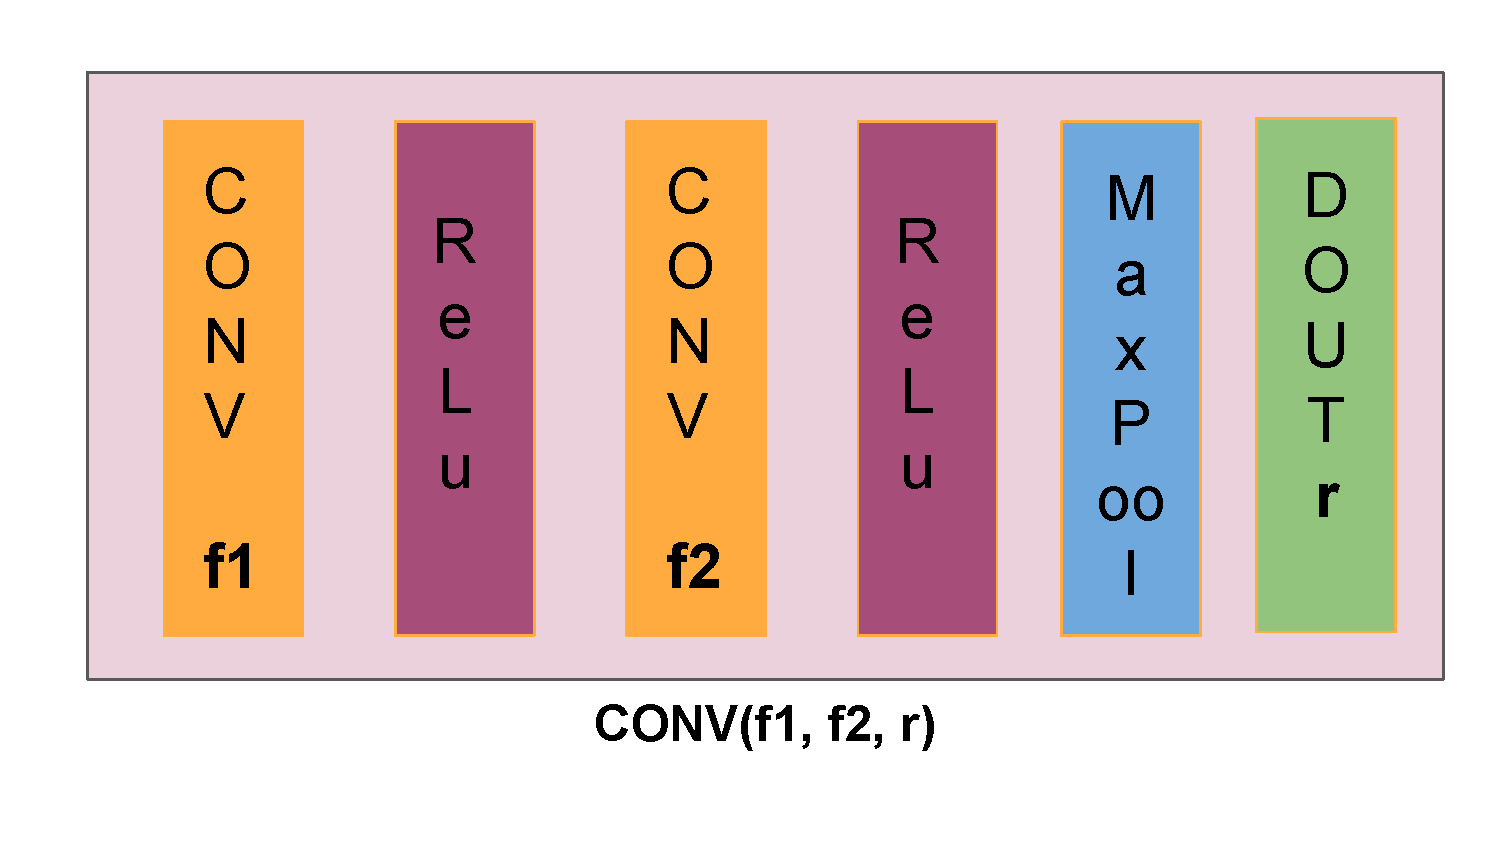
\includegraphics[scale=0.6]{Images/ConvB.pdf}
	\end{figure}
\end{minipage}
\hfill
\begin{minipage}{0.45\onecolwid}
\begin{center}
\textbf{FC Block$\textbf{(f1, A, r)}$}
\vspace*{0in}
\begin{itemize}
\item $\textbf{f1}$: Fully connected layer with $f1$ outputs
\item \textbf{$\textbf{A}$}: Activation function
\item \textbf{$\textbf{r}$}: Dropout ratio 
\end{itemize}
\end{center}

	\begin{figure}
	\centering
	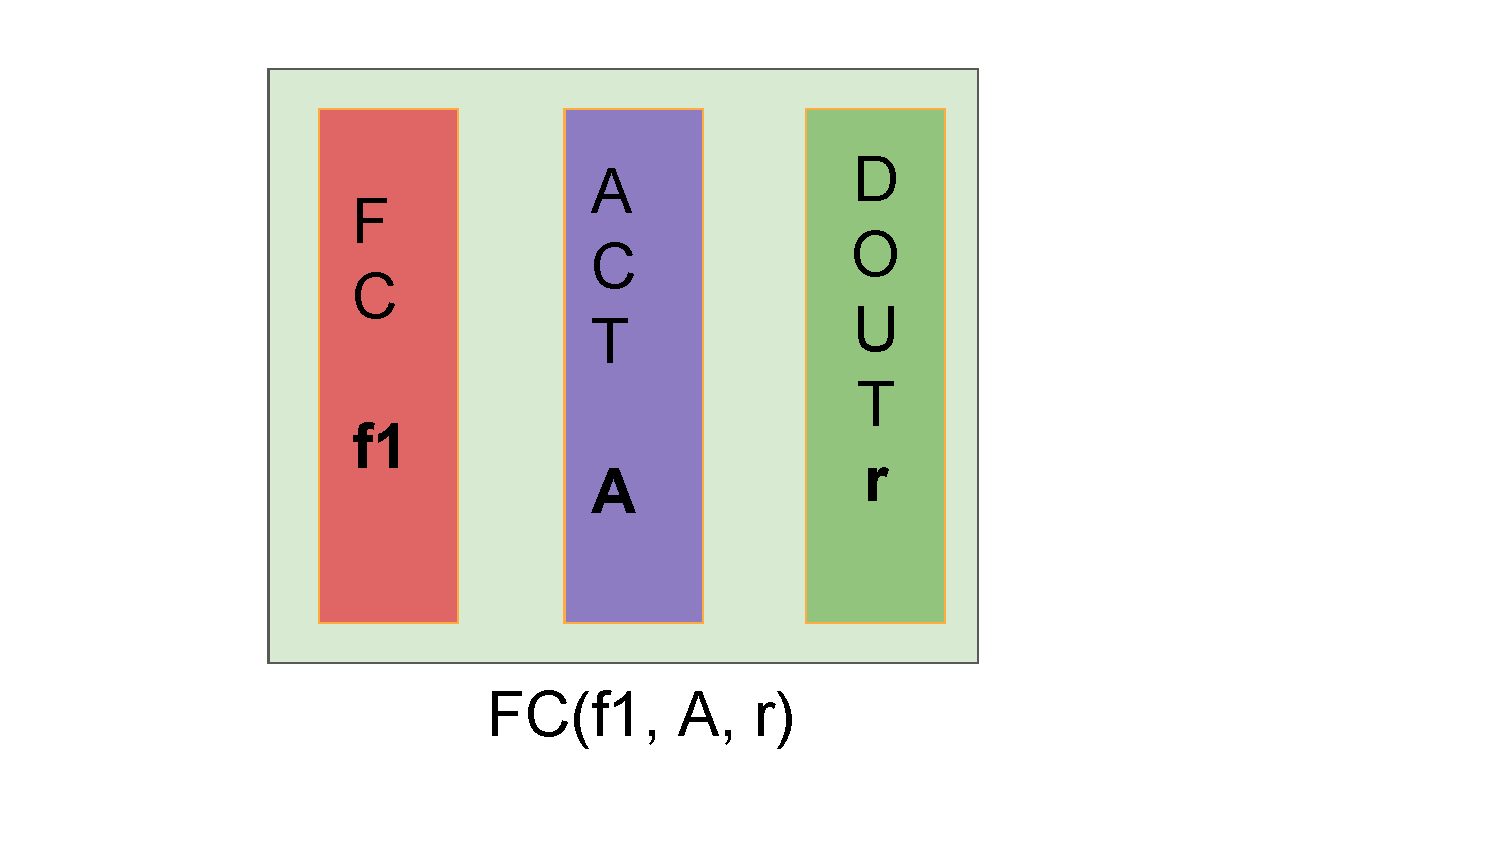
\includegraphics[scale=0.7, trim={30cm, 1cm, 30cm, 1cm}]{Images/FCB.pdf}
	\end{figure}
\end{minipage}
\hfill
\begin{minipage}{0.45\onecolwid}
\begin{itemize}
\item Kernel size $3\times 3$ for CONV Layer 
\item Stride size $2\times 2$ for MaxPool Layer 
\end{itemize}
\end{minipage}
\hfill
\begin{minipage}{0.45\onecolwid}
\begin{itemize}
\item Nesterov's  Gradient Descent (NGD) in CONV and FC layers
\end{itemize}
\end{minipage}

\end{block}

\begin{block}{$\textbf{\K}$ Architecture}

\[
\textbf{CONV}(\textbf{32}, \textbf{64}, \textbf{0.2})-\textbf{CONV}(\textbf{64}, \textbf{64}, \textbf{0.2}) - \]
\[ - \textbf{FC}(\textbf{512}, \textbf{ReLu}, \textbf{0.5}) - \textbf{FC}(\textbf{10}, \textbf{SoftMax}, \textbf{0})
\]

\end{block}

\begin{block}{Implemenation details}
	\begin{minipage}{0.5\onecolwid}
	\textbf{Data Preprocessing}
	\begin{itemize}
	\item Normalize values 
	\item Shift images with mean of training set
	\item Shift images by 10\% in vert. and hori. direction
	\item Flip images along vert. and hori. axes
	\end{itemize}
	\end{minipage}
	\hfill
	\begin{minipage}{0.5\onecolwid}
	\textbf{Epoch}
			\begin{itemize}
			\item Train on 300 epochs
			\item 0.98 split on training set 
			\item Each epoch trained on 49K images, validation on 1K images
			\end{itemize}
	\textbf{NGD parameters}: Learning rate = $10^{-3}$, Decay rate to $10^{-6}$ , momentum = 0.9

	\end{minipage}
\end{block}

\begin{block}{Experimental setup}

\begin{minipage}{0.4\onecolwid}
$\sim$10x faster comptuation 
\begin{itemize}
\item Amazon elastic compute instance (EC2)
\begin{itemize}
\item Nvidia GRID K520 GPU
\item Xeon E5-2670 processes 8 hyperthreads
\item 15 GiB RAM
\end{itemize}
\item $\mathsf{OpenBLAS}$ to optimize $\mathsf{NumPy}$
\item $\mathsf{CUDA}$ drivers with $\mathsf{CuDNN}$ library
\end{itemize}
\end{minipage}
\begin{minipage}{0.6\onecolwid}
\centering
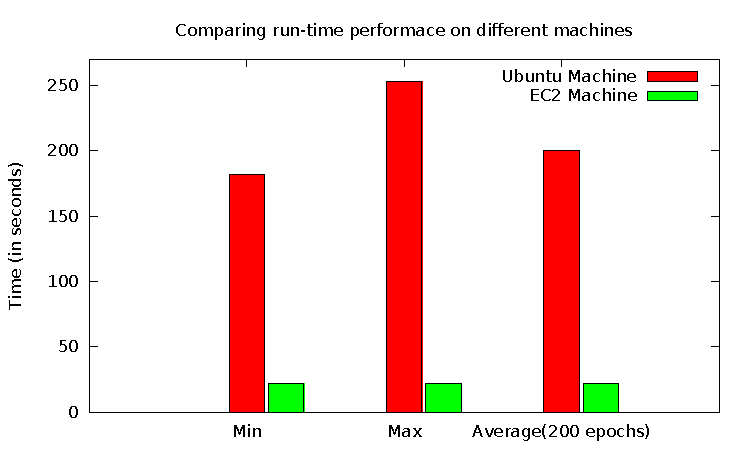
\includegraphics[scale=1.2]{Submissionlogs/RunTime.pdf}
\end{minipage}
\end{block}


\end{column} % End of the first column


\begin{column}{\sepwid}\end{column} % Empty spacer column
\begin{column}{\twocolwid} % Begin a column which is two columns wide (column 2)

\setbeamercolor{block alerted title}{fg=white,bg=UniBlue} % Colors of the highlighted block titles
\setbeamercolor{block alerted body}{fg=black,bg=white} % Colors of the body of blocks

\begin{alertblock}{Kaggle submissions report card}
\vspace*{0.3in}

	\begin{columns}[t,totalwidth=\twocolwid] % Split up the two columns wide column
		
		
		\begin{column}{0.4\twocolwid} %\vspace{-.6in} % The first column within column 2 (column 2.1)
		\begin{block}{Accuracy for all Kaggle submissions}
		
		\begin{figure}
				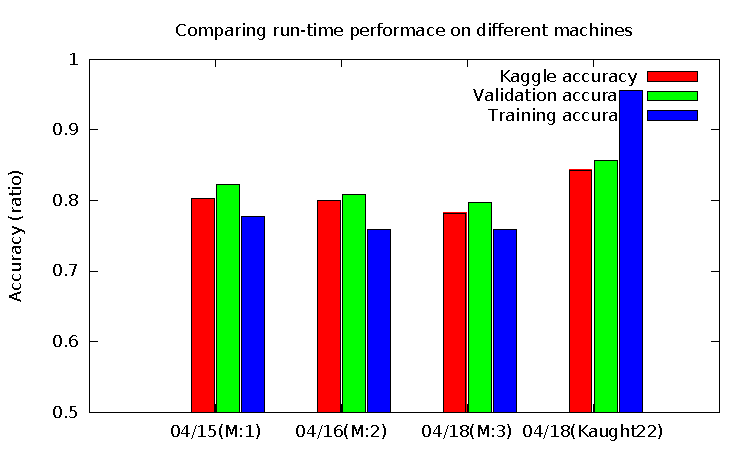
\includegraphics[scale=2.5]{Submissionlogs/KaggleReport.pdf}
				\caption{Trends of accuracy on training data and validation data on $\K$}
		\end{figure}			 
		
		\end{block}	
		\end{column}
		
		%\begin{column}{0.01\twocolwid}\end{column}
		
		\hfill
		\begin{column}{0.55\twocolwid}
		\begin{block}{Accuracy trends on $\K$}
		\begin{figure}
		\includegraphics[scale=2.5, page=4]{Submissionlogs/LogAcc.pdf}
		\caption{Trends of accuracy on training data and validation data on $\K$}
		\end{figure}
				
		\end{block}	
		
		\end{column}		
	\end{columns}
\end{alertblock}
\setbeamercolor{block alerted title}{fg=white,bg=dblue!70} % Colors of the highlighted block titles
\begin{columns}[t,totalwidth=\twocolwid] % Split up the two columns wide column

\begin{column}{\middlecolwid}\vspace{-.6in} % The first column within column 2 (column 2.1)


\setbeamercolor{block alerted body}{fg=black,bg=white} % Colors of the body of blocks
\medskip
\bigskip
\bigskip
\bigskip
\begin{alertblock}{Other Kaggle submissions}
\bigskip
\bigskip
\begin{itemize}
\item No mean shift data preprocessing. Rest data proprocessing identical to $\K$
\item Same epoch configuration as $\K$, number of epochs may vary
\item Same configuration for NGD as $\K$
\end{itemize}

\bigskip
\bigskip
\bigskip
\textbf{04/15 (M:1)}
\begin{itemize}
\bigskip
\item Identical to $\K$, aggressive dropout ratio= 0.25 on CONV Blocks 
\item Trained on 200 epochs
\end{itemize}
\bigskip
\bigskip
\bigskip
\textbf{04/16 (M:2)}
\begin{itemize}
\bigskip
\item Additional CONV Blocks
\[
\textbf{CONV}(\textbf{32}, \textbf{64}, \textbf{0.25})-\textbf{CONV}(\textbf{64}, \textbf{64}, \textbf{0.25}) - \textbf{CONV}(\textbf{128}, \textbf{64}, \textbf{0.25}) -\]
\[ - \textbf{FC}(\textbf{256}, \textbf{ReLu}, \textbf{0.5}) - \textbf{FC}(\textbf{10}, \textbf{SoftMax}, \textbf{0})
\]
\item Trained on 200 epochs
\end{itemize}
\bigskip
\bigskip
\bigskip
\textbf{04/18 (M:3)}
\begin{itemize}
\bigskip
\item Identical to $\K$, meek dropout ratio= 0.125 on CONV Blocks 
\item Trained on 300 epochs
\end{itemize}
\bigskip
\bigskip


\end{alertblock}
%----------------------------------------------------------------------------------------


%----------------------------------------------------------------------------------------
%	IMPORTANT RESULT
%----------------------------------------------------------------------------------------


%----------------------------------------------------------------------------------------


%----------------------------------------------------------------------------------------
%	MATHEMATICAL SECTION
%----------------------------------------------------------------------------------------

%----------------------------------------------------------------------------------------



\end{column} % End of the second column


\begin{column}{\middlecolwid}\vspace{-.6in} % The second column within column 2 (column 2.2) 
\medskip
\bigskip
\bigskip
\bigskip
\bigskip
\bigskip
\bigskip
\bigskip
%\begin{alertblock}{Worst Case Complexity}
%Exponential in size of input weighted regular game
%\begin{itemize}
%	\item Blow up due to single B\'uchi complementation step
%\end{itemize}
%\end{alertblock}
%\bigskip
%\bigskip
%----------------------------------
%          CONCLUSION
%----------------------------------
\begin{block}{Conclusion}
\textbf{Experimental setup}
\begin{itemize}
\bigskip
\item EC2 set up reduces runtime by $\sim$10x
\end{itemize}
\bigskip
\textbf{Hyper-parameter tuning }
\begin{itemize}
\bigskip
\item Adding more layers less beneficial
\item Too aggressive and too meek dropout regularization not helpful
\end{itemize}
\bigskip
\textbf{Data preprocessing}
\begin{itemize}
\bigskip
\item Mean shift improves accuracy drastically
\item Hori. and vert. flips makes model more sturdy
\end{itemize}

\end{block}

\begin{block}{Source Code}
\begin{center}
\url{https://github.com/HarshUpadhyay/COMP540_Project}
\end{center}

%\begin{center}
%	\includegraphics*[width=7cm]{Images/chart.png}
%\end{center}

\end{block}

\bigskip
\bigskip





\end{column} % End of the third column

\end{columns} % End of all the columns in the poster
\end{column}


\begin{column}{\startsepwidth}\end{column} % Empty spacer column
\end{columns}
\end{frame} % End of the enclosing frame

\end{document}
